\chapter{Results}
    In this chapter we present our results for the implementation of our pose estimation and the depth map acquired from \citetitle{luo2020consistent}~\cite{luo2020consistent}.
    We try to pinpoint the problems we encountered in our pipeline by comparing our results to the synthetic dataset 'lr kt2' from \citetitle{handa:etal:ICRA2014}~\cite{handa:etal:ICRA2014}.
    \section{pose optimization}
        Figure~\ref{fig:initial_reconstruction} shows our first valid results for one of our own videos. We were hoping to drastically improve on this results after optimizing the global poses.
        \begin{figure}[ht]
            \centering
            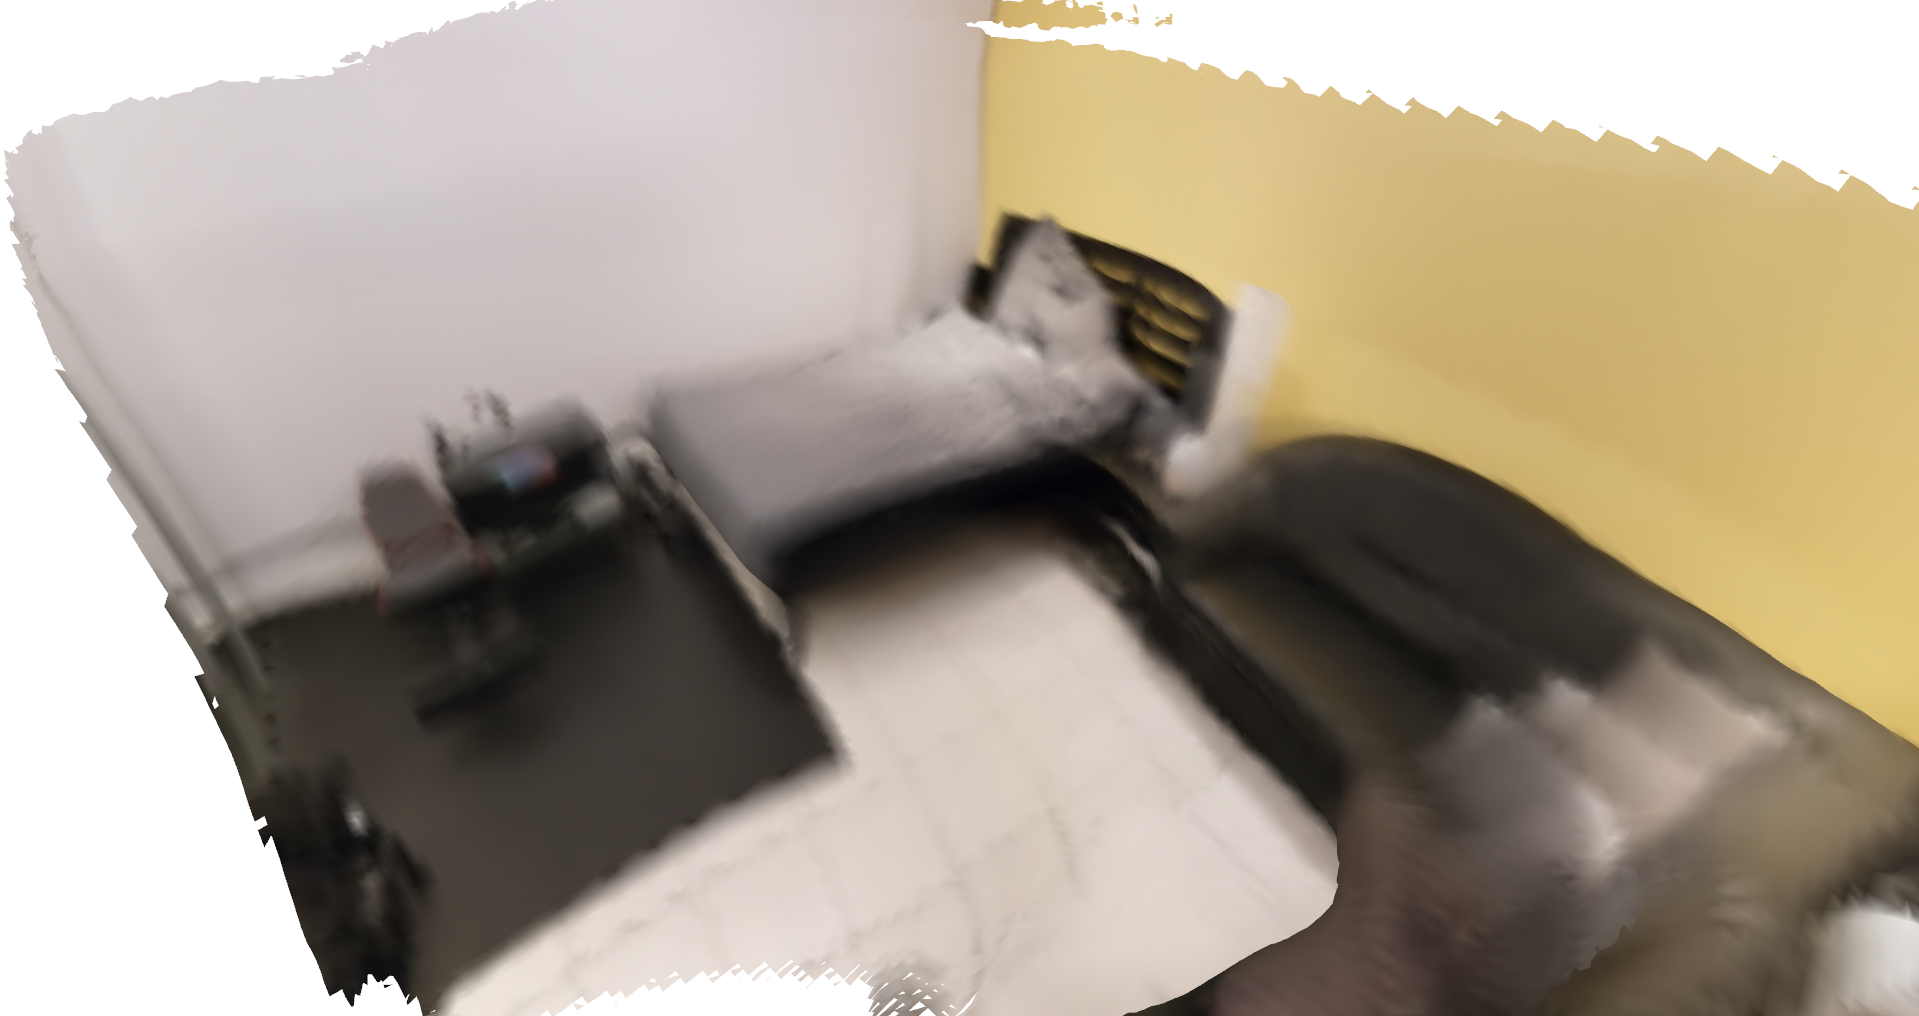
\includegraphics[width=.6\textwidth]{images/initial_reconstruction.png}
            \caption{Initial reconstruction on unoptimized pose estimates on one of our own videos.}
            \label{fig:initial_reconstruction}
        \end{figure}
        It turned out, that our method for the pose estimation described in chapter~\ref{sec:method_pose_optimization}, while not meant to be fast, was actually very computationally expensive. As the amount of frames increases, the number of valid frame pairs can potentially grow exponentially. In order to avoid computing for unreasonable amounts of time
        \begin{itemize}
            \item show initial reconstruction without optimization (kinda shitty)
            \item explain that for optimization reasons we now have to only look at a subset of frames (kinda like they keyframes in bundlefusion (without combining the chunks into one keyframe..)). and to make it fair, we compare initial reconstruction with the same frames as the optimized reconstruction.
            \item show initial reconstruction without and with optimization (both strided)
            \item compare and TRY to show, that it improved it in some way. the ground truth data should help here. hopefully we get a lower absolute trajectory error after the optimiziation. also some qualitative results (3d reconstruction screencaps).
            \item question if there even is a better set of extrinsics to combine the frames, leading to a potential other problem..
        \end{itemize}
    \section{Consistent Depth}
        \begin{itemize}
            \item maybe lead with a screenshot from the 3d reconstruction and a relevant frame from the video that shows, that corners are rounded and the depth is obviously flawed! (protein-tuete, ecken, meine wand die auch omegarund ist)
            \item describe how we compared the "consistent depth depth" to the ground truth --> leads to error heatmap that shows how off the depth estimate is
        \end{itemize}